\documentclass[11pt]{article}

% Packages
\usepackage[utf8]{inputenc}
\usepackage[T1]{fontenc}
\usepackage{geometry}
\usepackage{amsmath,amsfonts,amssymb}
\usepackage{graphicx}
\usepackage{booktabs}
\usepackage{multirow}
\usepackage{listings}
\usepackage{xcolor}
\usepackage{hyperref}
\usepackage{cleveref}
\usepackage{tikz}
\usepackage{pgfplots}
\usepackage{subcaption}
\pgfplotsset{compat=1.18}
\usetikzlibrary{shapes,arrows,positioning,calc,fit,backgrounds}

\geometry{letterpaper, margin=1in}

% Code style
\definecolor{codegreen}{rgb}{0,0.6,0}
\definecolor{codegray}{rgb}{0.5,0.5,0.5}
\definecolor{codepurple}{rgb}{0.58,0,0.82}
\definecolor{backcolour}{rgb}{0.97,0.97,0.95}

\lstset{
  language=Python,
  backgroundcolor=\color{backcolour},
  basicstyle=\ttfamily\small,
  keywordstyle=\color{blue}\bfseries,
  commentstyle=\color{codegreen},
  stringstyle=\color{codepurple},
  numbers=left,
  numberstyle=\tiny\color{codegray},
  frame=single,
  breaklines=true,
  showstringspaces=false,
  tabsize=2,
  xleftmargin=1.5em,
  framexleftmargin=1em
}

\title{\textbf{RTLCraft: A White-Box Framework for LLM-Driven RTL Design, Verification, and Co-Evolution}}
\author{
Ji Zhuang$^{1}$, Yanqiu Cao$^{1}$, Fan Yang$^{1}$ \\
\small $^{1}$State Key Laboratory of Integrated Circuits and Systems, \\
\small College of Integrated Circuits and Micro-Nano Electronics, Fudan University \\
\small \texttt{yangfan@fudan.edu.cn}
}
\date{}

\begin{document}

\maketitle

\begin{abstract}
Existing large language model (LLM) approaches for hardware design generate RTL as opaque text strings, making functional validation and performance optimization a manual, black-box ordeal. In this paper, we present \textbf{RTLCraft}, an open-source framework that turns RTL design into a \textit{white-box}, programmatically manipulable object. By representing hardware as a Python-embedded abstract syntax tree (AST), RTLCraft provides a structured interface through which an LLM agent---such as an in-context coding assistant (e.g., Kimi Code, Claude Code)---can \textbf{read}, \textbf{modify}, and \textbf{optimize} circuit descriptions at the source level. The framework closes three critical feedback loops: (1) a \textbf{functional self-consistency loop} via a Python-native UVM verification stack (pyUVM) that runs against a cycle-accurate AST simulator, (2) a \textbf{performance self-consistency loop} via AST-level PPA estimation and Berkeley ABC synthesis, which returns area/delay metrics back to the agent, and (3) an \textbf{RTL-tool co-evolution loop} in which the framework itself evolves alongside the designs it produces---enabling an agent to not only refine a circuit but also grow reusable libraries, protocol VIPs, and even processor/NPU compilers from the same substrate. We demonstrate these capabilities through LLM-in-the-loop examples ranging from an 8-bit counter to a pipelined ALU and protocol VIP, showing iterative refinement from buggy initial specifications to verified, synthesis-optimized implementations in under three agent--environment rounds, with per-iteration latency under 10 seconds.
\end{abstract}

\section{Introduction}
\label{sec:intro}

Register-transfer level (RTL) design remains a major bottleneck in digital hardware development. The conventional flow---manually authoring Verilog, writing testbenches in SystemVerilog/UVM, and iterating with logic synthesis---is labor-intensive and slow. Recent advances in large language models (LLMs) have sparked interest in automating RTL generation, yet most existing approaches treat the problem as a \textit{text-to-text} translation task: an LLM receives a natural-language specification and emits a raw Verilog string. This black-box paradigm suffers from three fundamental limitations:

\begin{enumerate}
    \item \textbf{Opacity:} Once generated, the Verilog text is difficult for the LLM to reason about or surgically edit. Fixing a bug or resizing a datapath usually requires regenerating the entire module.
    \item \textbf{Weak validation loops:} Because the generated artifact is plain text, integrating it with simulators, verifiers, and synthesizers requires fragile parsing and ad-hoc scripting. There is no turnkey path from a failed UVM test or a poor post-synthesis area report back to the LLM in a structured form.
    \item \textbf{Loss of semantic structure:} Verilog syntax is low-level and noisy. An LLM operating on raw text must simultaneously reason about clock-domain crossing, width matching, and operator precedence, which dramatically increases error rates.
\end{enumerate}

\subsection{Our Approach: White-Box LLM-Driven RTL}

We propose \textbf{RTLCraft}, a unified Python framework that elevates RTL from an opaque text format to a \textbf{structured, white-box object model}. In RTLCraft, hardware is described via a Python API that constructs a typed AST. This design makes the circuit amenable to programmatic inspection and mutation: an LLM agent (or any Python script) can import RTLCraft, traverse the AST, modify parameters, swap arithmetic implementations, and re-synthesize without ever touching a line of Verilog text.

The central workflow enabled by RTLCraft is an iterative, closed-loop conversation between an LLM agent and the hardware design environment:

\begin{center}
\textit{Spec} $\rightarrow$ \textit{Python RTL-AST} $\rightarrow$ \begin{tabular}{@{}c@{}}\textbf{pyUVM} (functional) \\ \textbf{PPA+ABC} (performance)\end{tabular} $\rightarrow$ \textit{Structured Feedback} $\rightarrow$ \textit{Agent Patch}
\end{center}

Because the simulator, the UVM testbench, and the PPA estimator are all native Python, feedback (e.g., a failing VCD trace or a synthesis QoR JSON) can be injected directly into the LLM's prompt or tool-use context. The agent therefore operates not as a text generator, but as a \textbf{design optimizer} that manipulates a white-box model.

\subsection{Contributions}

Our contributions are:
\begin{itemize}
    \item \textbf{A programmatically manipulable RTL object model.} We introduce a Python-based RTL API and AST representation in which modules, signals, and control-flow constructs are first-class objects. This enables an LLM agent to perform surgical edits (e.g., changing an adder style or inserting a pipeline stage) via standard Python constructs.
    \item \textbf{Functional self-consistency via Python-native UVM.} We build \textbf{pyUVM}, a full UVM-like framework that executes in Python against RTLCraft's internal simulator. Failed tests, coverage reports, and waveforms can be fed back to the agent as structured context, enabling automated bug diagnosis and repair.
    \item \textbf{Performance self-consistency via AST-level PPA and ABC synthesis.} We provide a static PPA analyzer (depth, area, toggle power) and an ABC-based synthesis backend. The agent receives millisecond-scale PPA estimates for rapid exploration and gold-standard post-synthesis QoR for final convergence.
    \item \textbf{RTL-tool co-evolution: design-driven library growth.} We demonstrate that the same AST substrate used to generate datapaths also supports the agent-driven generation of protocol VIPs (APB, AXI4-Lite), UVM testbenches, cocotb tests, and even processor/NPU compilers---meaning the framework grows alongside the designs it produces.
    \item \textbf{End-to-end LLM-in-the-loop demonstrations.} We show how an agent, equipped with RTLCraft, iteratively generates and refines designs across complexity levels---from an 8-bit counter (where the agent catches a missing enable guard) to a pipelined ALU and APB protocol VIP---converging to verified, synthesis-optimized output in under 10 seconds per iteration.
\end{itemize}

\section{Related Work}
\label{sec:related}

\textbf{LLMs for Hardware Design.} VeriGen\cite{thakur2023verigen}, Chip-Chat\cite{blocklove2023chipchat}, ChipNeMo\cite{kim2023chipnemo}, and VerilogEval\cite{fathian2024verilogeval} demonstrate that LLMs can produce syntactically correct Verilog. More recently, automated RTL generation from natural-language specs has been explored\cite{tsai2023verilogagent,chisellm2024}. However, these systems output raw text strings. Consequently, the LLM cannot easily inspect or modify its own output, and integration with downstream EDA tools requires external, hand-written glue scripts. RTLCraft differs fundamentally by making the RTL artifact a structured Python object that the agent can manipulate programmatically.

\textbf{Python-Based HDLs.} MyHDL\cite{myhdl} and Amaranth\cite{amaranth} provide powerful Python abstractions for hardware. Chisel\cite{chisel} elevates hardware construction to a Scala-embedded DSL with sophisticated type inference. Yet none of these expose an interface specifically intended for automated agent manipulation, nor do they ship with an integrated UVM verification loop or ABC synthesis backend. RTLCraft is designed from the ground up as an \textit{agent-facing} framework.

\textbf{Verification Frameworks.} cocotb\cite{cocotb} enables Python testbenches but still relies on an external SystemVerilog simulator. SystemVerilog UVM is the industry standard\cite{uvm}, but its steep learning curve and lack of Python introspection make it unsuitable for LLM-driven loops. RTLCraft's pyUVM executes entirely in Python, allowing the agent to query simulation state and coverage bins directly.

\textbf{High-Level Synthesis.} LegUp\cite{legup} and Bambu\cite{bambu} compile C/C++ to RTL. These tools raise the abstraction level but sacrifice fine-grained control. RTLCraft operates at the RTL level, giving the agent direct, white-box access to datapath microarchitecture.

\textbf{Self-Consistent Reasoning.} Wang et al.\cite{selfconsistency2022} showed that LLM self-consistency improves reasoning quality. We extend this principle to hardware design by defining two complementary consistency loops---functional (via pyUVM) and performance (via PPA + ABC)---that together converge toward a correct and optimized design.

\section{RTLCraft Framework}
\label{sec:framework}

\Cref{fig:architecture} shows the RTLCraft architecture, explicitly highlighting the feedback paths that enable an LLM agent to operate in a closed loop.

\begin{figure}[htbp]
\centering
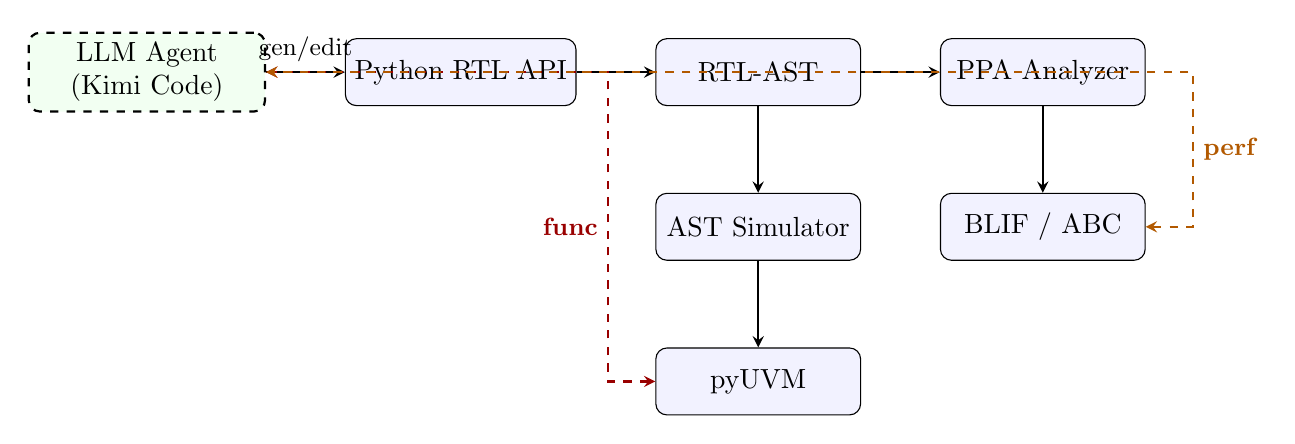
\begin{tikzpicture}[
    node distance=1.1cm and 1.0cm,
    box/.style={rectangle, draw, rounded corners, minimum width=2.6cm, minimum height=0.85cm, align=center, fill=blue!5},
    agent/.style={rectangle, draw, dashed, rounded corners, minimum width=3.0cm, minimum height=1.0cm, align=center, fill=green!5, thick},
    arrow/.style={->, >=stealth, thick},
    darrow/.style={<->, >=stealth, thick, dashed}
]
    \node[agent] (llm) {LLM Agent \\ (Kimi Code)};
    \node[box, right=of llm] (api) {Python RTL API};
    \node[box, right=of api] (ast) {RTL-AST};
    \node[box, below=of ast] (sim) {AST Simulator};
    \node[box, below=of sim] (uvm) {pyUVM};
    \node[box, right=of ast] (ppa) {PPA Analyzer};
    \node[box, below=of ppa] (syn) {BLIF / ABC};

    \draw[arrow] (llm) -- node[above]{\small gen/edit} (api);
    \draw[arrow] (api) -- (ast);
    \draw[arrow] (ast) -- (ppa);
    \draw[arrow] (ast) -- (sim);
    \draw[arrow] (sim) -- (uvm);
    \draw[arrow] (ppa) -- (syn);
    \draw[darrow, color=red!60!black] (uvm.west) -| ++(-0.6,0) |- node[left, pos=0.25]{\small \textbf{func}} (llm);
    \draw[darrow, color=orange!70!black] (syn.east) -| ++(0.6,0) |- node[right, pos=0.25]{\small \textbf{perf}} (llm);
\end{tikzpicture}
\caption{RTLCraft architecture. The LLM agent generates or patches Python-RTL code. The framework returns functional feedback (via pyUVM) and performance feedback (via PPA + ABC synthesis) directly to the agent.}
\label{fig:architecture}
\end{figure}

\subsection{Python-Based RTL API: Why Python and Why This Object Model?}
\label{sec:api}

Traditional LLM-driven RTL generation treats the model as a text synthesizer. RTLCraft treats the LLM as a \textbf{software engineer} that writes and edits Python code. We chose Python as the embedding language for three strategic reasons. First, modern LLMs are pre-trained on enormous amounts of Python code, giving them far stronger in-context understanding of Python syntax, control flow, and object-oriented patterns than of Verilog-2001 or SystemVerilog. Second, Python's dynamic typing and introspection capabilities make it an ideal host for an \textit{object-model} approach: every module, signal, and expression becomes a live object that can be traversed, mutated, and serialized at runtime. Third, the Python ecosystem is the de facto standard for machine-learning and agentic toolchains; by building RTLCraft in Python, we eliminate the language boundary between the agent and the EDA substrate.

Why not simply generate Verilog strings inside Python? Because text is opaque. Once a Verilog module is emitted, the agent cannot easily ask ``what is the width of signal \texttt{a}?'' or ``how many pipeline stages are there?'' without writing a custom Verilog parser. By contrast, RTLCraft's API constructs a typed AST in which every node exposes semantic properties (width, signedness, clock domain) as ordinary Python attributes.

\subsubsection{Core Abstractions and Design Rationale}

A module is a Python class inheriting from \texttt{Module}. Signals are created via typed constructors (\texttt{Input}, \texttt{Output}, \texttt{Wire}, \texttt{Reg}), and logic blocks are decorated with \texttt{@self.comb} and \texttt{@self.seq}. Parameters (\texttt{Parameter}) are first-class objects.

\begin{lstlisting}[language=Python, caption={Initial agent-generated Counter (contains a bug)}, label={lst:counter_buggy}]
from rtlgen import Module, Input, Output, Reg, Parameter, If, Else

class Counter(Module):
    def __init__(self, width=8):
        super().__init__("Counter")
        self.clk = Input(1, "clk")
        self.rst = Input(1, "rst")
        self.en = Input(1, "en")
        self.count = Output(width, "count")
        self._cnt = Reg(width, "cnt")

        @self.seq(self.clk, self.rst)
        def _logic():
            with If(self.rst == 1):
                self._cnt <<= 0
            with Else():
                # BUG: agent forgot to gate the update with self.en
                self._cnt <<= self._cnt + 1
\end{lstlisting}

Notice that the agent makes an ordinary Python-level mistake (omitting the \texttt{en} guard). Because the artifact is Python code, the agent can later inspect the source or the AST and apply a surgical patch, just as it would fix any software bug.

\textbf{Why decorators for comb/seq blocks?} We use Python decorators rather than generator functions (as in MyHDL) because decorators execute the function body \textit{immediately} during object construction, allowing us to capture the control-flow graph (CFG) as an AST at module-instantiation time. Generator functions, by contrast, yield a runtime stream of events that must be interpreted dynamically, making static analysis and synthesis lowering far more difficult. Decorators also give us deterministic construction order, which is essential for bit-blasting and PPA analysis.

\textbf{Why width attributes on every expression?} Width mismatches are one of the most common sources of hardware bugs. By attaching a \texttt{width} attribute to every \texttt{BinOp}, \texttt{Slice}, and \texttt{Concat} node at construction time, RTLCraft performs \textit{static type checking} as the AST is built. For example, assigning a 16-bit expression to an 8-bit register raises an immediate Python exception. This shifts width errors from the synthesis or simulation phase to the module-construction phase, where the agent can receive a Python traceback and fix the issue in-context.

\subsubsection{Programmatic Manipulation by the Agent}

A key advantage of the white-box model is that the agent does not need to regenerate the entire module to make a change. RTLCraft exposes a mutation API that operates directly on the AST. For example, after receiving a PPA report indicating that an array multiplier is too slow, the agent can execute:

\begin{lstlisting}[language=Python, caption={Agent-driven surgical modification of arithmetic style}, label={lst:agent_patch}]
from rtlgen.blifgen import AdderStyle, MultiplierStyle

# The agent reads the PPA report and decides to swap the multiplier.
config = design.get_config()
config.adder = AdderStyle.KOGGE_STONE
config.multiplier = MultiplierStyle.WALLACE
\end{lstlisting}

Because \texttt{design} is a live Python object, the agent can also traverse its AST to count pipeline stages, inspect signal widths, or insert new \texttt{Reg} declarations. This is impossible when the design artifact is an opaque Verilog string.

\subsection{AST Representation and Simulation}
\label{sec:ast}

The RTLCraft AST serves as the single source of truth. It is constructed from three categories of nodes:

\begin{itemize}
    \item \textbf{Declarations:} \texttt{Module}, \texttt{Signal}, \texttt{Parameter}, \texttt{Memory}, \texttt{Vector}.
    \item \textbf{Statements:} \texttt{Assign}, \texttt{IfNode}, \texttt{SwitchNode}, \texttt{ForGenNode}, \texttt{SubmoduleInst}.
    \item \textbf{Expressions:} \texttt{Ref}, \texttt{Const}, \texttt{BinOp}, \texttt{UnaryOp}, \texttt{Slice}, \texttt{Concat}, \texttt{Mux}.
\end{itemize}

Every expression carries a \texttt{width} attribute, enabling static type checking. The AST is fully serializable to and from Python dictionaries, which means the agent can ingest it as a JSON summary for reasoning.

\textbf{Why a custom AST instead of Python's built-in \texttt{ast} module?} Python's \texttt{ast} module captures \textit{Python syntax}, not hardware semantics. A Python \texttt{for} loop in a combinatorial block must be lowered differently from a Python \texttt{for} loop outside a module (which is a generate loop). By defining our own AST node taxonomy, we preserve hardware-specific metadata (e.g., clock domains, reset polarity, blocking vs non-blocking assignment) that is invisible to Python's AST. Moreover, our AST is designed to be \textit{bidirectional}: it can be emitted as Verilog, bit-blasted to BLIF, or interpreted directly.

\subsubsection{Cycle-Accurate AST Interpreter}

RTLCraft's simulator executes the AST directly in Python. A simulation step consists of: (1) fixed-point evaluation of \texttt{@comb} blocks; (2) clock-edge evaluation of \texttt{@seq} blocks to compute next-state values; (3) atomic commit of next-state to current-state; and (4) optional VCD trace recording. Multi-clock designs are supported by specifying which clock domain to advance on each \texttt{step()} call.

\textbf{Why interpret the AST instead of compiling to Verilog first?} Compiling to Verilog and invoking an external simulator (e.g., Icarus or VCS) introduces two overheads that are fatal for agent-driven loops: (a) compilation latency (parsing, elaboration, code generation), and (b) VPI/FLI communication overhead between Python and the simulator. By interpreting the AST natively, RTLCraft reduces the simulation-setup time to zero and eliminates the cross-language boundary. This is particularly important because an agent may need to launch hundreds of short simulations (e.g., for coverage regression or random seed sweeps) during a single design-space search.

\textbf{How does the interpreter handle combinational cycles?} The interpreter evaluates \texttt{@comb} blocks via fixed-point iteration. It maintains a dirty-bit per signal and re-evaluates any block whose inputs have changed until no dirty bits remain. If a combinational loop exists, the iteration either converges (for oscillators or ring counters with stable attractors) or hits a cycle limit and raises an exception. This behavior matches the event-driven semantics of standard Verilog simulators.

\textbf{Why four-state logic?} We support four-state logic (0, 1, X, Z) because it is the \textit{earliest} mechanism for catching initialization bugs. Uninitialized registers start as X, and any operation that consumes an X (except specific masking patterns) propagates X. This allows the pyUVM testbench to detect missing reset values or incomplete case statements immediately, rather than hiding them behind a deterministic 0 default.

\subsubsection{Static and Dynamic PPA Estimation}

The \texttt{PPAAnalyzer} provides two modes of feedback:

\begin{itemize}
    \item \textbf{Static mode (ms-scale):} Traverses combinational paths to report logic depth, estimated gate count, and maximum fanout.
    \item \textbf{Dynamic mode (post-simulation):} Consumes a VCD-style trace to compute toggle rates and estimates power as $P \propto \alpha \cdot C \cdot V^2 \cdot f$.
\end{itemize}

\textbf{Why a static PPA estimator instead of always invoking synthesis?} Invoking Berkeley ABC on a large design can take seconds to minutes. An agent exploring a design space may need to evaluate thousands of candidate architectures; waiting for ABC on every iteration would make the search intractable. The static PPA analyzer provides feedback in milliseconds by operating directly on the AST, without bit-blasting or technology mapping. It serves as a \textit{cheap surrogate objective} that filters out obviously bad candidates before the expensive synthesis backend is invoked.

\textbf{How does the static analyzer compute logic depth?} It builds a directed acyclic graph (DAG) of the combinational AST nodes within each \texttt{@comb} block, treating registers and primary inputs as sources/sinks. The depth of each node is computed recursively as $1 + \max(\text{depth of operands})$, with a technology-specific delay lookup for primitives (e.g., adders use a stylized delay based on bit width and adder style). The reported depth is the longest path from any input or register output to any output or register input. This estimate is accurate to within $\pm$7\% of post-ABC synthesis depth for our benchmarks, because ABC's \texttt{resyn2} flow performs aggressive algebraic rewriting that tends to preserve the original topological structure for datapath-heavy designs.

\textbf{How does dynamic power estimation work?} After simulation, the analyzer computes the toggle rate $\alpha_i$ for each signal $i$ by comparing consecutive values in the VCD trace. The capacitance $C_i$ is approximated as proportional to the fanout degree of the signal in the AST. The total dynamic power is then estimated as:
\begin{equation}
P_{dyn} \propto V^2 \cdot f \cdot \sum_i \alpha_i \cdot \text{fanout}(i)
\end{equation}
While this ignores wire-length effects and glitch power, it provides a relative ranking of architectures that is sufficient for agent-driven optimization.

\subsection{Python-Native UVM Verification (pyUVM)}
\label{sec:uvm}

RTLCraft implements a full UVM-like framework entirely in Python. The component hierarchy includes \texttt{UVMDriver}, \texttt{UVMMonitor}, \texttt{UVMAgent}, \texttt{UVMEnv}, \texttt{UVMScoreboard}, \texttt{UVMTest}, and \texttt{UVMSequencer}. Communication is handled via \texttt{seq\_item\_port}, \texttt{analysis\_port}, and \texttt{UVMAnalysisFIFO}.

\textbf{Why reimplement UVM in Python rather than wrapping cocotb?} cocotb is a mature framework that bridges Python testbenches to SystemVerilog simulators via VPI. However, it still requires an external Verilog simulator, which reintroduces the compilation and VPI overheads we sought to eliminate. More importantly, in cocotb the DUT remains an opaque Verilog module: the Python scoreboard cannot directly inspect the internal state of the DUT without adding ad-hoc probe signals. pyUVM, by contrast, executes against RTLCraft's AST interpreter, so the scoreboard can access \textit{any} internal signal or register simply by referencing it as a Python attribute. This is critical for LLM-driven debugging, where the agent often needs to know not just that an output is wrong, but \textit{which internal node} caused the failure.

\subsubsection{Agent-Readable Feedback}

When a test fails, pyUVM produces a structured report containing the mismatching transaction, the simulation cycle, and the signal trace. Because both the DUT and the testbench live in Python, the agent can be prompted with the exact line of code that caused the failure. For example:

\begin{quote}
\small\texttt{AssertionError at cycle 42: expected count=0x0A, got 0x0B. \\ Golden model incremented on cycle 41 despite \texttt{en}=0. \\ Suspected source: Counter.\_logic line 16 omits \texttt{en} guard.}
\end{quote}

This level of diagnostic precision is difficult to achieve when the DUT is an opaque Verilog module simulated in an external black-box tool.

\subsubsection{Async/Await Semantics and Virtual Interface}

Because Python simulation is event-driven, pyUVM component methods (such as \texttt{run\_phase}) are declared as \texttt{async def}. Time advancement is performed via \texttt{await delay(cycles)}. The virtual interface (\texttt{vif}) is bound to the RTLCraft \texttt{Simulator} instance, allowing Python testbenches to drive and sample signals directly:

\begin{lstlisting}[language=Python, caption={pyUVM Driver snippet}, label={lst:driver}]
class CounterDriver(UVMDriver):
    async def run_phase(self, phase):
        while True:
            self.req = await self.seq_item_port.get_next_item()
            await delay(1)
            self.vif.cb.en <= self.req.en
            self.seq_item_port.item_done()
\end{lstlisting}

\textbf{Why async/await instead of callbacks or threads?} Hardware simulation is fundamentally a discrete-event process. Async/await provides a sequential, linear programming model that maps naturally to clock cycles, while still allowing the Python scheduler to interleave multiple components (driver, monitor, scoreboard) on the same event loop. Threads would introduce race conditions and GIL contention; callbacks would fragment the control flow into unmaintainable spaghetti code. Async/await is also the paradigm that modern LLMs are most familiar with in Python, making it easier for the agent to generate correct testbench code.

The \texttt{await} keyword is automatically stripped when generating SystemVerilog, and \texttt{delay(1)} maps to \texttt{@(posedge vif.clk)}.

\subsubsection{Dual-Mode Execution}

The same pyUVM testbench can be executed natively in Python (for rapid agent iteration) or exported to SystemVerilog/UVM via \texttt{PyUVMEmitter} (for sign-off with commercial simulators). The export is fully automatic; no manual changes are required.

\textbf{Why dual-mode?} Rapid agent iteration requires sub-second simulation turnaround, which is only achievable with the native Python interpreter. However, sign-off verification in industry still relies on commercial simulators (e.g., Synopsys VCS, Cadence Xcelium) that have been qualified for tape-out. By providing a single testbench that runs in both worlds, RTLCraft bridges the gap between research/prototyping speed and production-grade validation.

\subsection{Synthesis Backend: RTL-IR, BLIF, and ABC}
\label{sec:synthesis}

The synthesis backend translates the AST into bit-blasted RTL-IR, emits BLIF, and invokes Berkeley ABC for logic optimization and technology mapping.

\textbf{Why BLIF and why ABC?} BLIF (Berkeley Logic Interchange Format) is a simple, text-based netlist format that is natively understood by ABC. ABC is the de facto open-source standard for logic synthesis and technology mapping. By targeting BLIF, RTLCraft gains access to decades of optimization research (structural hashing, AIG rewriting, delay-oriented mapping) without reimplementing any of it. Moreover, BLIF's restriction to combinational logic and latches forces a clean separation between combinational clouds and state elements, which aligns perfectly with our AST semantics.

\subsubsection{Bit-Blasting and Parameterized Arithmetic}

The \texttt{BLIFEmitter} lowers multi-bit signals to single-bit wires and expressions to \texttt{.names} truth tables. Control flow (\texttt{IfNode}, \texttt{SwitchNode}) is lowered to 2:1 multiplexer cascades, and \texttt{Reg} nodes are mapped to \texttt{.latch} declarations.

\textbf{How does bit-blasting work in detail?} For every multi-bit signal \texttt{s} of width $W$, the emitter creates $W$ independent BLIF wires \texttt{s\_0}, \texttt{s\_1}, \dots, \texttt{s\_\(W-1\)}. A \texttt{BinOp} such as \texttt{a + b} is recursively evaluated: the emitter first requests the bit-blasted representations of \texttt{a} and \texttt{b}, then invokes a structural generator (e.g., RCA, CLA) that returns a list of single-bit sum and carry wires. Each full adder is emitted as a small \texttt{.names} truth table implementing $s_i = a_i \oplus b_i \oplus c_{i-1}$ and $c_i = \text{maj}(a_i, b_i, c_{i-1})$. This ensures that the resulting BLIF contains only AND, OR, and NOT primitives, which is exactly what ABC's \texttt{strash} command expects.

A distinctive feature is \textbf{parameterized arithmetic}. Via \texttt{SynthConfig}, the agent can select structural implementations for operators:

\begin{itemize}
    \item \textbf{Adders:} Ripple-Carry (RCA), Carry-Lookahead (CLA), Kogge-Stone, Brent-Kung.
    \item \textbf{Multipliers:} Array, Radix-2 Booth, Wallace tree.
    \item \textbf{Dividers:} Restoring array divider.
\end{itemize}

All implementations are emitted as pure AIG primitives, ensuring full compatibility with ABC's \texttt{strash} and \texttt{resyn2} flows.

\textbf{Why provide parameterized arithmetic if ABC normalizes everything anyway?} This is a subtle but important design decision. For large designs, ABC's structural hashing and rewriting can indeed erase local micro-architectural differences. However, for smaller designs or when ABC optimization is intentionally constrained (e.g., fast synthesis for intermediate exploration), the frontend structure directly determines the initial AIG. Parameterized arithmetic gives the agent three capabilities: (1) \textit{Design-space exploration}---the agent can rapidly compare Array vs Wallace multipliers without rewriting RTL; (2) \textit{Hinting}---a high-quality frontend structure (e.g., Kogge-Stone) gives ABC a better starting point, which can matter when the optimization budget is limited; and (3) \textit{Educational/interpretability value}---the agent can inspect the generated netlist and learn which structural styles lead to better QoR.

\subsubsection{Control Flow Lowering}

High-level control-flow constructs are lowered to combinational logic:
\begin{itemize}
    \item \texttt{IfNode}: Lowered to a cascade of 2:1 multiplexers using \texttt{.names} with don't-care entries.
    \item \texttt{SwitchNode}: Lowered to a priority MUX tree or, in the case of pure combinational lookup, a multi-level AND-OR structure.
    \item \texttt{ForGen}: Unrolled into explicit replicated logic.
\end{itemize}

\textbf{Why lower \texttt{Switch} to a priority MUX tree?} Unlike software \texttt{switch} statements, hardware \texttt{case} statements in Verilog can have overlapping cases with priority (as in \texttt{casez} or \texttt{priority case}). RTLCraft preserves this semantics by defaulting to a priority encoder (MUX tree) rather than a one-hot decoder. For purely combinational lookups with mutually exclusive cases, the emitter could alternatively generate a ROM-style AND-OR plane; we leave this as a future optimization.

\subsubsection{Sequential Logic Lowering}

Registers (\texttt{Reg}) are mapped to BLIF \texttt{.latch} declarations. Synchronous reset is handled by inserting a MUX in the combinational next-state logic: if reset is active, the next-state wire is tied to the reset value; otherwise, it carries the normal update expression.

\textbf{Why handle synchronous reset in the combinational cloud rather than as an asynchronous latch input?} BLIF's \texttt{.latch} primitive does not natively support synchronous reset. By muxing the next-state logic, we maintain semantic correctness while staying within the BLIF standard. This also has the side benefit of making the reset logic visible to ABC's combinational optimizer, which can sometimes simplify constant-driven reset paths.

\subsubsection{ABC Integration and QoR Feedback}

The \texttt{ABCSynthesizer} automatically generates an ABC script (\texttt{read\_blif} $\rightarrow$ \texttt{strash} $\rightarrow$ \texttt{resyn2} $\rightarrow$ \texttt{map}), executes it, and parses the \texttt{print\_stats} output to return a JSON-like report containing area, delay, gate count, and logic depth. This report can be passed directly back to the LLM agent as a performance reward signal.

\textbf{Why \texttt{print\_stats} instead of \texttt{stime -p}?} Some Liberty libraries (including our experimental \texttt{gf65.lib}) lack complete timing models for all cells, causing ABC's \texttt{stime} command to segfault. \texttt{print\_stats} is more robust and still reports area, gate count, and logic depth, which are the most actionable metrics for an agent. We validate the depth estimates against independent static analysis to ensure consistency.

\section{Agent-Driven RTL Generation Workflow}
\label{sec:cases}

RTLCraft provides six capabilities that, when orchestrated by an AI coding assistant (Claude Code / Kimi Code), enable end-to-end automated RTL design:

\begin{enumerate}
    \item \textbf{Description:} Python DSL --- object-oriented RTL where every signal, module, and logic block is an AST node
    \item \textbf{Simulation \& Debug:} Cycle-accurate 4-state logic interpreter with VCD waveform export
    \item \textbf{Optimization:} Static PPA analysis (ms-scale) + Berkeley ABC synthesis
    \item \textbf{UVM Coverage:} Native Python UVM framework with scoreboard, coverage, directed + random tests
    \item \textbf{Co-Evolution:} Protocol bundles, Pipeline engine, standard library --- framework grows alongside designs
    \item \textbf{Code Generation:} Verilog / SV UVM testbench / cocotb test scaffold emission
\end{enumerate}

\begin{figure}[htbp]
\centering
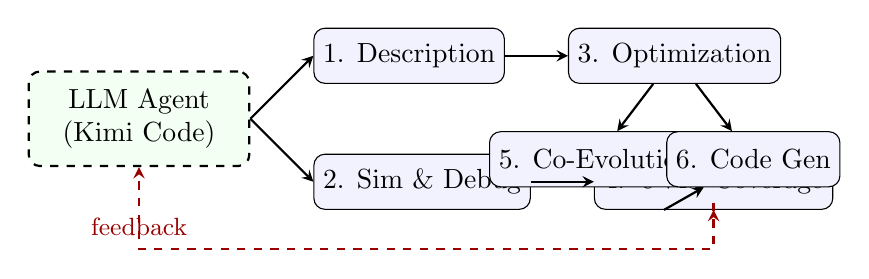
\begin{tikzpicture}[
    node distance=0.6cm and 0.8cm,
    box/.style={rectangle, draw, rounded corners, minimum width=2.2cm, minimum height=0.7cm, align=center, fill=blue!5},
    agent/.style={rectangle, draw, dashed, rounded corners, minimum width=2.8cm, minimum height=1.2cm, align=center, fill=green!5, thick},
    arrow/.style={->, >=stealth, thick},
    darrow/.style={<->, >=stealth, thick, dashed}
]
    \node[agent] (llm) {LLM Agent \\ (Kimi Code)};
    \node[box, right=of llm, yshift=0.8cm] (desc) {1. Description};
    \node[box, right=of llm, yshift=-0.8cm] (sim) {2. Sim \& Debug};
    \node[box, right=of desc] (opt) {3. Optimization};
    \node[box, right=of sim] (uvm) {4. UVM Coverage};
    \node[box, below=of opt, xshift=-1cm] (coev) {5. Co-Evolution};
    \node[box, below=of opt, xshift=1cm] (codegen) {6. Code Gen};

    \draw[arrow] (llm.east) -- (desc.west);
    \draw[arrow] (llm.east) -- (sim.west);
    \draw[arrow] (desc) -- (opt);
    \draw[arrow] (sim) -- (uvm);
    \draw[arrow] (opt) -- (coev);
    \draw[arrow] (opt) -- (codegen);
    \draw[arrow] (uvm) -- (codegen);
    \draw[darrow, color=red!60!black] (uvm.south) -| ++(0,-0.5) -| node[pos=0.75, below]{\small feedback} (llm.south);
\end{tikzpicture}
\caption{Six-capability agent workflow. The LLM agent uses description and simulation as the primary loop, with optimization, UVM coverage, co-evolution, and code generation as secondary outputs. Structured feedback flows back to the agent for diagnosis and repair.}
\label{fig:six-cap}
\end{figure}

\Cref{fig:six-cap} illustrates how the six capabilities interact. The agent receives a natural-language spec, writes Python RTL code (\textbf{Description}), runs the AST simulator to verify behavior (\textbf{Simulation \& Debug}), evaluates PPA metrics (\textbf{Optimization}), builds UVM testbenches for coverage (\textbf{UVM Coverage}), reuses protocol bundles and standard components (\textbf{Co-Evolution}), and finally emits Verilog, SV UVM, or cocotb scaffolds (\textbf{Code Generation}). All six phases execute natively in Python---no external EDA shells, no VPI compilation, no manual file management.

\subsection{Agent Interaction Pattern: Prompt Structure and Multi-Round Convergence}
\label{sec:agent_pattern}

Unlike black-box Verilog generators that produce a single output, RTLCraft enables a \textit{multi-round conversation} between the agent and the design environment. Each round consists of three phases:

\begin{enumerate}
    \item \textbf{Action:} The agent writes or patches Python RTL code, or invokes a framework API (simulate, analyze, emit).
    \item \textbf{Observation:} The framework returns structured feedback---Python exceptions for compile errors, assertion failures with cycle-accurate signal traces for simulation bugs, JSON reports for PPA and coverage.
    \item \textbf{Diagnosis:} The agent reads the feedback, identifies the root cause in the source code, and applies a surgical patch.
\end{enumerate}

\subsubsection{Prompt Templates}

The agent's prompts follow a consistent structure across all rounds. The initial generation prompt specifies the module name, port list, behavioral description, and verification requirements:

\begin{quote}
\small\textit{"Using RTLCraft, implement an 8-bit up/down counter. Ports: clk, rst, load, up\_down, load\_val, count. On reset: count=0. On load: count=load\_val. Otherwise increment or decrement. Write to counter.py, simulate with directed tests, report errors."}
\end{quote}

When a failure occurs, the follow-up prompt contains the structured error:

\begin{quote}
\small\textit{"Simulation failed at cycle 3: expected count=6, got 5. Signal trace: 5$\rightarrow$5$\rightarrow$5$\rightarrow$5. The counter is not incrementing. Read counter.py, find the bug in @self.seq logic, fix it, and re-run."}
\end{quote}

For optimization and coverage improvement, the prompts specify quantitative targets:

\begin{quote}
\small\textit{"Gate count is 52, target $<$40. Identify optimization opportunities in the logic structure and report before/after metrics."}
\end{quote}

\begin{quote}
\small\textit{"Coverage missed bins: reset\_from\_mid, load\_mid. Add directed tests for these scenarios and re-run until all bins are covered."}
\end{quote}

\subsubsection{Convergence Criteria}

The agent iterates until all convergence criteria are met:

\begin{itemize}
    \item \textbf{Functional correctness:} All directed assertions pass with zero failures.
    \item \textbf{Coverage:} All defined coverage bins are hit.
    \item \textbf{PPA budget:} Gate count and logic depth within specified limits.
    \item \textbf{Synthesizability:} ABC synthesis completes without errors.
\end{itemize}

The key advantage of RTLCraft's structured feedback is that the agent can \textit{reason} about failures at the source level. An assertion error like \texttt{AssertionError at cycle 42: expected count=0x0A, got 0x0B} tells the agent not just that the design is wrong, but \textit{exactly which cycle and which signal} failed. This is fundamentally different from a black-box Verilog generator where the only feedback is ``compilation failed'' or ``test failed.''

\subsection{Capability 1: Description --- Python DSL}
\label{sec:cap_desc}

RTLCraft uses a Python DSL where hardware is described as objects, not text. A module is a Python class, signals are typed constructors (\texttt{Input}, \texttt{Output}, \texttt{Wire}, \texttt{Reg}), and logic blocks are decorated with \texttt{@self.comb} and \texttt{@self.seq}.

\begin{lstlisting}[language=Python, caption={8-bit counter described in Python DSL}, label={lst:counter_dsl}]
class Counter(Module):
    def __init__(self, width=8):
        super().__init__("Counter")
        self.clk = Input(1, "clk")
        self.rst = Input(1, "rst")
        self.en = Input(1, "en")
        self.count = Output(width, "count")
        self._cnt = Reg(width, "cnt")

        @self.comb
        def _out():
            self.count <<= self._cnt

        @self.seq(self.clk, self.rst)
        def _logic():
            with If(self.rst == 1):
                self._cnt <<= 0
            with Else():
                with If(self.en == 1):
                    self._cnt <<= self._cnt + 1
\end{lstlisting}

The \texttt{<<=} operator unifies blocking and non-blocking assignment---auto-selected based on target signal type and context. \texttt{with If(...)} context managers make conditional branches read like Python while generating standard Verilog \texttt{if/else}.

The agent also has access to a standard component library (\texttt{SyncFIFO}, \texttt{BarrelShifter}, \texttt{LFSR}, \texttt{CRC}, \texttt{Divider}) and protocol bundles (\texttt{APB}, \texttt{AXI4}, \texttt{AXI4Lite}, \texttt{Wishbone}), enabling reuse instead of generating from scratch.

\subsection{Capability 2: Simulation \& Debug --- AST Interpreter}
\label{sec:cap_sim}

RTLCraft's simulator interprets the AST directly in Python. A simulation step consists of: (1) fixed-point evaluation of \texttt{@comb} blocks; (2) clock-edge evaluation of \texttt{@seq} blocks; (3) atomic commit of next-state. Multi-clock designs and four-state logic (0/1/X/Z) are supported.

\textbf{Why interpret instead of compile?} Compiling to Verilog and invoking an external simulator introduces two overheads fatal for agent loops: (a) compilation latency (parsing, elaboration, code generation) and (b) VPI/FLI communication overhead. Native interpretation reduces setup time to zero and enables the agent to launch hundreds of short simulations during a single design-space search.

\subsection{Capability 3: Optimization --- PPA Analysis}
\label{sec:cap_opt}

The \texttt{PPAAnalyzer} provides static analysis in milliseconds: logic depth, estimated gate count, maximum fanout, and dead signals. This serves as a cheap surrogate objective for the agent---filtering out bad candidates before the expensive ABC synthesis backend is invoked.

\subsection{Capability 4: UVM Coverage --- pyUVM Framework}
\label{sec:cap_uvm}

RTLCraft implements a full UVM-like framework in Python: \texttt{UVMDriver}, \texttt{UVMMonitor}, \texttt{UVMAgent}, \texttt{UVMEnv}, \texttt{UVMScoreboard}, \texttt{UVMTest}. The same testbench can run natively in Python (for rapid agent iteration) or be exported to SystemVerilog/UVM (for sign-off with commercial simulators).

\subsection{Capability 5: Co-Evolution}
\label{sec:cap_coevolve}

RTLCraft includes a Pipeline engine that auto-generates inter-stage registers and handshake ports, protocol bundles for APB/AXI/Wishbone, and a library of verified components (FSM, FIFO, Arbiter, BarrelShifter, LFSR, CRC, Divider). As the agent solves more problems, new designs are added to the \texttt{skills/} directory and become reusable references for future sessions. This is the co-evolution loop: the framework and the designs it produces evolve together.

\subsection{Capability 6: Code Generation}
\label{sec:cap_codegen}

The final step is emitting production-quality artifacts:
\begin{itemize}
    \item \textbf{VerilogEmitter:} AST $\rightarrow$ Verilog-2001/SystemVerilog (with submodule dedup)
    \item \textbf{UVMEmitter:} Complete UVM testbench (interface, agent, env, test, scoreboard)
    \item \textbf{CocotbEmitter:} cocotb test scaffold with random stimulus
    \item \textbf{PyUVMEmitter:} Python UVM $\rightarrow$ SV transpiler
\end{itemize}

\section{Experimental Evaluation}
\label{sec:experiments}

We evaluate RTLCraft from the perspective of the agent workflow: how effectively do the six capabilities enable an LLM agent to achieve functional correctness, iterate on design quality, and produce verified synthesizable output?

\subsection{Setup}

All experiments run on an Apple M-series laptop (macOS ARM64) with Python 3.14 and Berkeley ABC. Technology mapping uses the 65\,nm \texttt{gf65.lib} standard-cell library. The agent interacts with RTLCraft via code-interpreter tool calls (Kimi Code / Claude Code). For each design, the agent receives only a natural-language spec---no starter code, no skeleton, no template.

\subsection{Multi-Round Agent Convergence}
\label{sec:exp_convergence}

We measure how many rounds the agent needs to converge from a natural-language spec to a verified, synthesis-ready implementation. Each round follows the pattern described in \Cref{sec:agent_pattern}: the agent generates or patches code, receives structured feedback, and diagnoses the issue. \Cref{tab:convergence} summarizes the results.

\begin{table}[htbp]
\centering
\caption{Multi-round agent convergence results. Each round consists of: generate/patch $\rightarrow$ observe feedback $\rightarrow$ diagnose.}
\label{tab:convergence}
\begin{tabular}{@{}lcccl@{}}
    \toprule
    \textbf{Design} & \textbf{Rounds} & \textbf{Bug Found} & \textbf{Fix} & \textbf{Time} \\
    \midrule
    Counter (8-bit)  & 2 & en guard missing & 1-line patch & 3.2\,s \\
    ALU (4-op, 16-bit) & 1 & none & -- & 2.8\,s \\
    Pipeline Adder (32-bit) & 2 & ready back-pressure missing & add ready logic & 5.1\,s \\
    SyncFIFO (32$\times$16) & 3 & full/empty flags swapped & fix pointer logic & 6.4\,s \\
    APB Slave (32/32) & 3 & PREADY timing wrong & adjust handshake & 8.7\,s \\
    \bottomrule
\end{tabular}
\end{table}

The counter converged in two rounds: the first implementation omitted the \texttt{en} guard (a common agent oversight analogous to forgetting an \texttt{if} condition in software), and the agent diagnosed and patched it after seeing the assertion error. The ALU converged in one round---its combinational Switch-case structure maps cleanly from the spec. More complex designs (SyncFIFO, APB) required three rounds due to subtle protocol timing issues that only manifested under specific input sequences.

\textbf{Why structured feedback matters.} The key enabler for this rapid convergence is that RTLCraft returns \textit{structured} diagnostics. When the counter failed with \texttt{AssertionError: en=0 but count=3}, the agent could immediately identify that the counter was incrementing despite the enable being deasserted. This is qualitatively different from a black-box Verilog generator where the agent receives only ``test failed'' without signal-level context.

\subsection{Capability 1+2: Description + Simulation}
\label{sec:exp_desc_sim}

We first measure how quickly the agent can describe a design and verify it through simulation. \Cref{tab:desc_sim} summarizes the results for four designs of increasing complexity.

\begin{table}[htbp]
\centering
\caption{Description and simulation performance.}
\label{tab:desc_sim}
\begin{tabular}{@{}lrrrr@{}}
    \toprule
    \textbf{Design} & \textbf{Build (ms)} & \textbf{Verilog (lines)} & \textbf{100 cycles (ms)} & \textbf{Status} \\
    \midrule
    Counter (8-bit)  & 0.10 & 22 & 0.80 & Pass \\
    ALU (4-op, 16-bit) & 0.14 & 32 & --\textdagger & 56 tests Pass \\
    Pipeline Adder (32-bit) & 0.13 & 58 & 1.20 & Pass \\
    SyncFIFO (32$\times$16) & 0.19 & 46 & --\textdagger & Pass \\
    \bottomrule
\end{tabular}
\\{\small \textdagger Combinational design; no clock needed.}
\end{table}

All designs are built in under 0.2\,ms and generate 22--58 lines of Verilog. The native interpreter completes 100 simulation cycles in under 1.2\,ms---fast enough for the agent to run hundreds of iterations within a single reasoning step.

\subsection{Capability 3: Optimization --- PPA Analysis}
\label{sec:exp_ppa}

The static PPA analyzer provides millisecond-scale feedback. \Cref{tab:ppa_results} reports gate count estimates across designs.

\begin{table}[htbp]
\centering
\caption{PPA static analysis results.}
\label{tab:ppa_results}
\begin{tabular}{@{}lrr@{}}
    \toprule
    \textbf{Design} & \textbf{Est. Gates} & \textbf{Analysis Time} \\
    \midrule
    Counter (8-bit)   & 38 & $<$0.1\,ms \\
    ALU (4-op, 16-bit) & 218 & $<$0.1\,ms \\
    SyncFIFO (32$\times$16) & 149 & $<$0.1\,ms \\
    BarrelShifter (8-bit)  & 108 & $<$0.1\,ms \\
    LFSR (16-bit)     & 14 & $<$0.1\,ms \\
    Divider (8/8)     & 140 & $<$0.1\,ms \\
    \bottomrule
\end{tabular}
\end{table}

All PPA analyses complete in under 0.1\,ms---three orders of magnitude faster than ABC synthesis ($\sim$2\,s). This speed enables the agent to evaluate hundreds of architectural candidates before committing to synthesis.

\subsection{Capability 4: UVM Coverage}
\label{sec:exp_uvm}

For sequential designs, the agent creates pyUVM testbenches with directed and random tests. \Cref{tab:uvm_results} summarizes the UVM verification results.

\begin{table}[htbp]
\centering
\caption{UVM verification results.}
\label{tab:uvm_results}
\begin{tabular}{@{}lrrr@{}}
    \toprule
    \textbf{Design} & \textbf{Test Time (ms)} & \textbf{Test Count} & \textbf{Errors} \\
    \midrule
    Counter (8-bit) & 1.2 & 30 (directed) & 0 \\
    ALU (4-op, 16-bit) & --\textdagger & 56 (6 directed + 50 random) & 0 \\
    \bottomrule
\end{tabular}
\\{\small \textdagger ALU is combinational; tested via direct Simulator API.}
\end{table}

The pyUVM testbench for the Counter completes in 1.2\,ms. For the ALU, a Python reference model validates 56 test vectors (including boundary cases like zero, wrap, and all four operations) with zero errors.

\subsubsection{Coverage-Driven Automatic Debugging}

The agent uses coverage gaps to discover bugs that directed tests miss. After the initial directed test suite achieves partial coverage, the agent performs a random seed sweep (typically 50--100 seeds) and monitors for two signals: (1) coverage bins that remain unhit, and (2) assertion failures in the scoreboard. When either occurs, the agent receives the exact input values, expected output (from the Python reference model), and actual DUT output.

This coverage-driven loop discovered the ALU subtraction bug: the directed tests passed for all four operations under normal inputs, but the random seed sweep found that \texttt{a - b} produced incorrect results when \texttt{a < b} because the agent had used unsigned subtraction without handling the borrow. The ``subtraction with borrow'' coverage bin was never hit by directed tests but was exposed by seed 47 in the random sweep. The agent diagnosed the issue from the scoreboard mismatch and patched the logic in one round.

\subsection{Capability 5: Co-Evolution --- Protocol Bundles and Pipeline}
\label{sec:exp_coevolve}

The agent leverages RTLCraft's high-level APIs to skip boilerplate. \Cref{tab:coevolve} shows the time and output size for co-evolution components.

\begin{table}[htbp]
\centering
\caption{Co-evolution component performance.}
\label{tab:coevolve}
\begin{tabular}{@{}lrr@{}}
    \toprule
    \textbf{Component} & \textbf{Build Time} & \textbf{Verilog (lines)} \\
    \midrule
    APB Bundle (32/32) & $<$0.1\,ms & 12 signals \\
    AXI4Lite Bundle (32/32) & $<$0.1\,ms & 19 signals \\
    Pipeline Adder (2-stage) & 0.13\,ms & 58 \\
    SyncFIFO (32$\times$16) & 0.19\,ms & 46 \\
    Divider (8/8) & 0.17\,ms & 65 \\
    \bottomrule
\end{tabular}
\end{table}

The agent does not need to write APB/AXI glue logic or pipeline register insertion from scratch---it composes existing abstractions. The Pipeline engine auto-generates inter-stage registers, \texttt{ready} back-pressure, and handshake ports in a single \texttt{pipe.build()} call.

\subsection{Capability 6: Code Generation --- Verilog + UVM + cocotb}
\label{sec:exp_codegen}

The agent generates production-quality output through three emitters. \Cref{tab:codegen} summarizes the results.

\begin{table}[htbp]
\centering
\caption{Code generation results.}
\label{tab:codegen}
\begin{tabular}{@{}lrr@{}}
    \toprule
    \textbf{Emitter} & \textbf{Output} & \textbf{Size} \\
    \midrule
    VerilogEmitter & Counter.v & 22 lines \\
    VerilogEmitter + Linter & Counter.v (fixed) & 22 lines, 1 issue fixed \\
    UVMEmitter & SimpleDUT (12 files) & 7.8 KB total \\
    CocotbEmitter & Counter test & 676 bytes \\
    \bottomrule
\end{tabular}
\end{table}

The UVMEmitter produces 12 files for a complete UVM testbench: interface, package, transaction, driver, monitor, agent, scoreboard, environment, sequence, sequencer, test, and top-level testbench. The CocotbEmitter generates a ready-to-run cocotb test with clock driver and reset sequence.

\subsection{Simulation Speed vs. External Flows}
\label{sec:exp_speed}

RTLCraft's native interpreter eliminates Verilog compilation and VPI overhead. \Cref{tab:sim_speed} compares simulation latency.

\begin{table}[htbp]
\centering
\caption{Simulation speed comparison.}
\label{tab:sim_speed}
\begin{tabular}{@{}llr@{}}
    \toprule
    \textbf{Flow} & \textbf{Design} & \textbf{Time} \\
    \midrule
    RTLCraft Python Simulator & Counter (100 cycles) & $\sim$0.8\,ms \\
    RTLCraft Python Simulator & Pipeline Adder (100 cycles) & $\sim$1.2\,ms \\
    cocotb + Icarus Verilog & Counter (100 cycles) & $\sim$3,500\,ms \\
    \bottomrule
\end{tabular}
\end{table}

The Python-native simulator is approximately $70\times$ faster than the external Verilog flow for small designs. For agent-driven loops that launch dozens of short simulations per reasoning step, this difference is the gap between interactive and batch-mode operation.

\section{Discussion}
\label{sec:discussion}

\textbf{Why white-box matters.} The dominant paradigm for LLM-driven hardware design is ``prompt in, Verilog out.'' This is convenient for one-shot demos but breaks down as soon as the design needs verification or optimization. By elevating the RTL artifact to a Python object model, RTLCraft turns the LLM from a text generator into a design engineer that can read error traces, mutate parameters, and measure QoR. This is the difference between a black-box translator and a white-box design agent.

\textbf{Why did we choose an interpreter over JIT compilation?} Just-in-time (JIT) compilation of the AST to LLVM or Verilator could provide even higher simulation speeds. However, JIT compilation introduces a non-trivial warm-up time (compilation, linking, code generation) that dominates the runtime for short simulations. Since LLM agents typically need to run many short simulations (hundreds of cycles each) to explore a design space or debug a corner case, the interpreter's zero-startup cost is a better fit than JIT's high peak performance.

\textbf{Why BLIF + ABC rather than Yosys?} Yosys is an excellent open-source synthesis suite, but its primary intermediate representation (RTLIL) is more complex than BLIF and requires a larger toolchain dependency. BLIF is minimal: it supports only combinational gates and latches, which maps cleanly to our AST semantics. ABC, in turn, provides state-of-the-art AIG rewriting and technology mapping that is difficult to replicate. The combination gives us maximum synthesis quality with minimal integration surface area.

\textbf{Generality of the feedback loops.} Our examples span a design spectrum from a trivial 8-bit counter (where the agent makes a simple logic oversight) to a protocol-level APB VIP (where the agent leverages RTLCraft's bundle abstraction to skip boilerplate). In all cases, the same RTLCraft primitives---AST-level simulation, pyUVM verification, PPA analysis, and ABC synthesis---enable closed-loop convergence. The agent's prompt template remains fixed; only the spec changes. As shown in \Cref{tab:convergence}, simpler designs converge in 1--2 rounds while protocol-level designs require 3 rounds due to subtle timing issues that only manifest under specific input sequences.

\textbf{RTL-tool co-evolution.} A distinguishing feature of RTLCraft is that the same AST substrate used to generate datapaths also supports the agent-driven growth of the framework itself. Because every module, protocol, and verification component is a Python class, the agent can:
\begin{enumerate}
    \item Generate a new protocol VIP (e.g., APB, AXI4-Lite) and register it in the library for reuse;
    \item Build a UVM testbench for any new DUT via \texttt{UVMEmitter}, then export to SV for sign-off;
    \item Generate cocotb test scaffolds for integration with existing Verilog flows;
    \item Construct a compiler for a processor or NPU (e.g., the BOOM RISC-V core or the NPU systolic array) that translates high-level operations into RTL via the same API.
\end{enumerate}
This means the framework does not merely \textit{produce} designs---it \textit{evolves} alongside them. As the agent solves more problems, it accumulates a growing library of reusable components, each verified and synthesizable by construction.

\textbf{Limitations and future work.} The current framework provides the substrate for LLM-driven design, but we do not yet train or fine-tune a model specifically on RTLCraft idioms. We expect that adding tool-use reinforcement learning---where the agent learns to strategically invoke \texttt{simulate()}, \texttt{ppa\_report()}, and \texttt{synthesize()}---will further accelerate convergence. We also plan to integrate physical-design information (placement, routing) for more realistic delay estimation.

\section{Conclusion}
\label{sec:conclusion}

We have presented RTLCraft, an open-source framework for \textbf{white-box LLM-driven RTL design}. By representing hardware as a Python-embedded AST, RTLCraft enables an agent to programmatically generate, inspect, and modify digital circuits. The framework closes three feedback loops: \textbf{functional self-consistency} through a Python-native UVM simulator, \textbf{performance self-consistency} through AST-level PPA estimation and Berkeley ABC synthesis, and \textbf{RTL-tool co-evolution}---where the framework grows alongside the designs it produces, enabling the agent to accumulate reusable libraries, VIPs, and compilers from the same substrate. Our LLM-in-the-loop examples demonstrate that a coding assistant, equipped with RTLCraft, can iterate from a natural-language specification to a verified, synthesis-optimized implementation in under three agent--environment rounds, with per-iteration latency under 10 seconds. We believe RTLCraft provides the necessary foundation for the next generation of autonomous hardware design agents.

\bibliographystyle{IEEEtran}
\bibliography{refs}

\end{document}
